\section{Hardware}
\label{section:hardware}

The hardware used in this work was a mobile 3D scanner called "lemonbot", shown in \cref{fig:lemonbot}. This scanner was developed to perform the acquisitions, and the goal was to build a platform that had minimum interference with the environment (for example, no cables are required), mobile (lightweight and easy to transport) and did not require the presence of the operator. Therefore, the robot was all packed into a tripod which also has a battery capable of powering all the systems. The control is made via a remote connection through the router, which is specially useful to make the repetitive task of acquisitions faster and more agile. 

\begin{figure}[p]
    
    \centering
    \includegraphics[height=20cm]{lemonbot}

    \caption{Lemonbot mobile 3D scanner}
    \label{fig:lemonbot}
\end{figure}

This robot has, in total, seven components: three of which are the essencial components for the acquisitions: the 2D laser scanner, the camera and the pan-tilt unit, or PTU and the other four components form the infrastructure: the minicomputer, the wireless router, the battery pack and finally the tripod. Each of these components are described in detail in the following lines.

\subsubsection{2D Laser Scanner}

One of the objectives of this work is to use different 2D laser scanners to study the performance of the reconstruction and calibration algorithms and to evaluate if not every laser scanner is fit for this application. So, three laser scanners were chosen: the SICK~LMS200, the Hokuyo~UTM30LX and the Hokuyo~URG04. Each of the laser scanners differ in their characteristics, like the size, price, range and error. In \cref{table:laserscanner-characteristics}, all three laser scanners can be compared and in \cref{fig:laserscanners} are shown.

\begin{table}[h]
    \caption{Comparison of the three laser scanners used, based on the data provided by the manufacturers.}

    \begin{tabu}{@{}>{\bfseries}X[l,m] X[c] X[c] X[c]@{}}
        \toprule

            & SICK LMS~100
            & Hokuyo UTM~30LX
            & Hokuyo URG04 \\
        \toprule

        \everyrow{\midrule}

        Aperture angle &
            \SI{270}{\degree} &
            \SI{270}{\degree} &
            \SI{240}{\degree} \\
        
        
        Angular resolution &
            \SI{0.25}{\degree} &
            \SI{0.25}{\degree} &
            \SI{0.36}{\degree} \\
        
        
        Scanning frequency &
            \SI{10}{\hertz} &
            \SI{40}{\hertz} &
            \SI{10}{\hertz} \\
        

        Maximum range &
            \SI{20}{\meter}  &
            \SI{30}{\meter}  &
            \SI{5.6}{\meter} \\
        

        Systematic error &
            \SI{+-40}{\milli\meter} &
            not available &
            not available \\
        
        
        Statistical error &
            \SI{20}{\milli\meter} &
            \SI{30}{\milli\meter} &
            \SI{30}{\milli\meter} \\
        

        Dimensions (\si{\milli\meter^3}) &
            \num{152x102x106} &
            \num{60x60x87} &
            \num{60x60x87} \\
        

        Weight &
            \SI{1100}{\gram} &
            \SI{370}{\gram} &
            \SI{160}{\gram} \\
        
        \everyrow{}

        Power consumption &
            \SI{<12}{\watt} &
            \SI{8.4}{\watt} &
            \SI{2.5}{\watt} \\

        \bottomrule
    \end{tabu}

    \label{table:laserscanner-characteristics}
\end{table}


\begin{figure}[h]
    
    \centering
    \begin{subfigure}{0.3\textwidth}
        \centering
        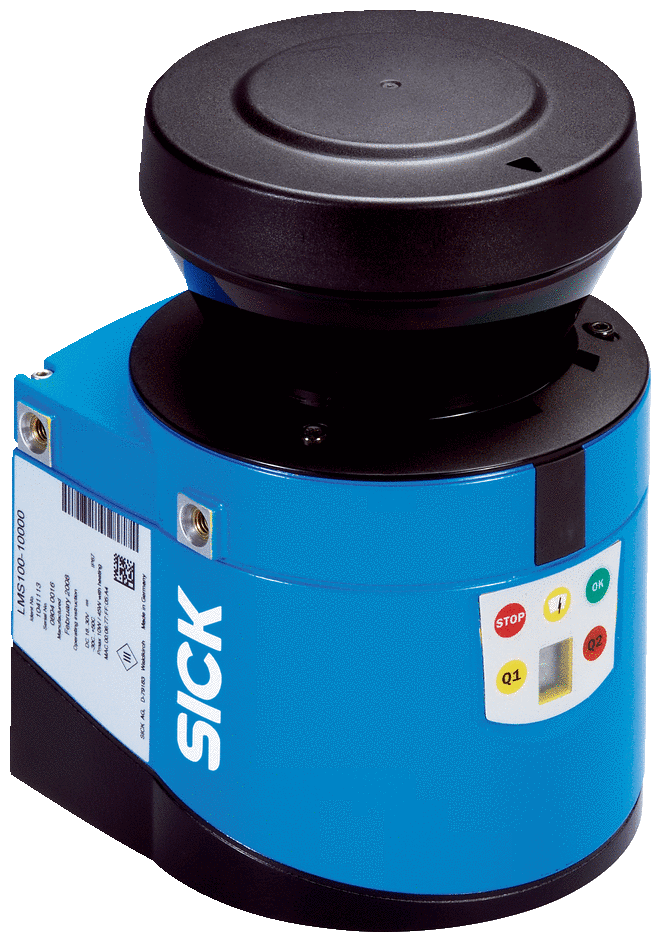
\includegraphics[height=4cm]{sick-lms100}
        \caption{SICK LMS100}
        \label{fig:sick-lms100}
    \end{subfigure}%
    \begin{subfigure}{0.3\textwidth}
        \centering
        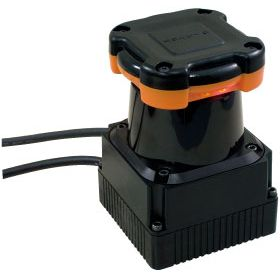
\includegraphics[height=4cm]{hokuyo-utm30lx}
        \caption{Hokuyo UTM30LX}
        \label{fig:hokuyo-utm30lx}
    \end{subfigure}%
    \begin{subfigure}{0.3\textwidth}
        \centering
        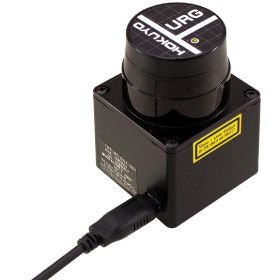
\includegraphics[height=4cm]{hokuyo-urg04}
        \caption{Hokuyo URG04}
        \label{fig:hokuyo-urg04}
    \end{subfigure}

    \caption{Laser scanners used.}
    \label{fig:laserscanners}

\end{figure}

\subsubsection{Camera}

The camera used in this work was a PointGrey Flea3 FL3-GE-28S4 Camera (\cref{fig:pointgrey-flea3}), which is extensively used in industrial and traffic applications. The high quality of the images, the programming interface and it's compact size and weight makes it perfect for computer vision applications in industrial environment. The most relevant characteristics are represented on the \cref{table:pointgrey-flea3-characteristics}.

\begin{figure}[h]
    \centering
    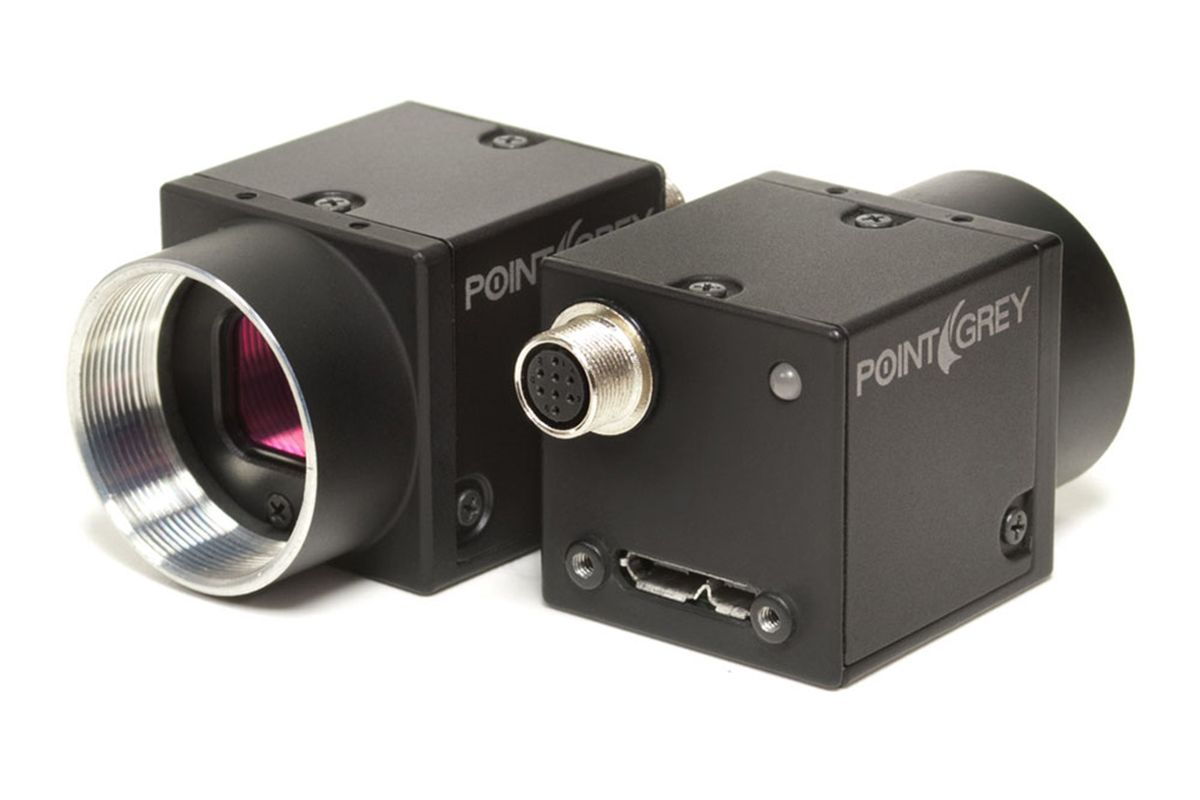
\includegraphics[width=0.5\textwidth]{pointgrey-flea3}
    \caption{PointGrey Flea3 FL3-GE-28S4}
    \label{fig:pointgrey-flea3}
\end{figure}

\begin{table}[h]

    \caption{Characteristics of the PointGrey Flea3 FL3-GE-28S4 Camera}

    \centering
    \begin{tabu} spread 0.2\textwidth {>{\bfseries}X[l] X[r]}
        \toprule

        Resolution  & $1920 \times 1448$    \\
        Framerate   & 15 fps                \\
        Pixels      & \SI{2.8}{\mega P}     \\
        Color       & Yes                   \\
        Interface   & GigE Vision           \\
        Power       & \SIrange{12}{24}{\volt} \\
        Dimensions  & \SI{29 x 29 x 30}{\milli\meter} \\
        \bottomrule
    \end{tabu}

    \label{table:pointgrey-flea3-characteristics}

\end{table}

\subsubsection{Pan Tilt Unit}

Both the laser and camera are placed on top of a pan and tilt unit for their movement. The selected PTU was the FLIR PTU-D46 (\cref{figure:ptu-d46}), which is a compact and light module with the characteristics shown in \cref{table:ptu-characteristics}.


\begin{table}[h]
    \caption{FLIR PTU-D46 characteristics.}

    \centering
    \begin{tabu} spread 0.15\textwidth {>{\bfseries}X[l] X[r]}
        \toprule
        Pan range & \SI{+-159}{\degree} \\
        Tilt range & \SIrange{-47}{+31}{\degree} \\
        Maximum payload weight & \SI{4}{\kilo\gram} \\
        Angular resolution & \SI{0.0032}{\degree} \\
        Communication & serial interface \\
        Size & small \\
        \bottomrule
    \end{tabu}

    \label{table:ptu-characteristics}
\end{table}

\begin{figure}[h]
    \centering
    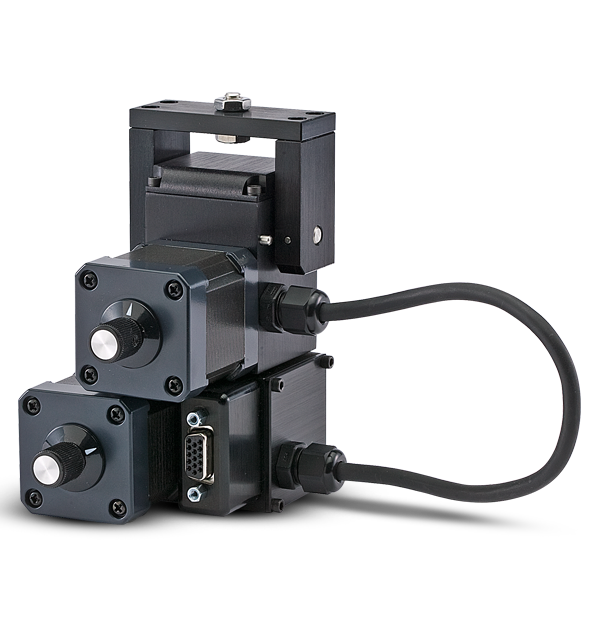
\includegraphics[width=0.5\textwidth]{ptu-d46}
    \caption{FLIR PTU-D46}
    \label{figure:ptu-d46}
\end{figure}
